\documentclass[12pt]{article}
\usepackage{amsmath}
\usepackage{graphicx}
\usepackage{hyperref}
\usepackage[utf8]{inputenc}
\usepackage{geometry}
\usepackage{mathtools}
\usepackage{empheq}
\usepackage{listings}
\usepackage{xcolor}
\usepackage{minted}
\definecolor{LightGray}{gray}{0.9}

\graphicspath{ {./assets/} }
\geometry{margin=0.75in}

\title{CHEN 364 HW 1}
\author{Mark Levchenko}
\date{January 2023}

\begin{document}
\maketitle

\begin{enumerate}

% Problem 1
    \item Problem 1
    \begin{enumerate}
        \item 
        \begin{align*}
            -r_A V_{\mathrm{CSTR}} &= F_{A0} - F_A \\
            F_A &= C_A v_0 \\
            C_A &= 0.01 C_{A0} \\
            F_A &= 0.01 C_{A0} v_0 \\
            -r_A &= k = 0.05 \\
            C_{A0} &= 0.5 \\
            F_{A0} &= 5 \\
            v_0 &= 10 \\
            V_{\mathrm{CSTR}} &= \frac{5 - 0.01 \cdot 0.5 \cdot 10}{0.05} \\
            \Aboxed{V_{\mathrm{CSTR}} &= 99 \mathrm{dm}^3}
        \end{align*}

        PFR:
        \begin{align*}
            \frac{dF_A}{dV_{\mathrm{PFR}}} &= r_A \\
            dF_A &= r_A dV_{\mathrm{PFR}} \\ 
            \int^{F_A}_{F_{A0}} dF_A &= \underset{V}{\int} r_A dV_{\mathrm{PFR}} \\ 
            -r_A &= k \\
            \int^{F_A}_{F_{A0}} dF_A &= \underset{V}{\int} -k dV_{\mathrm{PFR}} \\ 
            F_A - F_{A0} &= -k V_{\mathrm{PFR}} \\
            V_{\mathrm{PFR}} &= \frac{F_A - F_{A0}}{-k}
        \end{align*}
        The above equation is equivalent to the design equation for the CSTR in this problem. $r_A$ does not change with $C_A$, and the result is that the reaction rate does not change along the length of the PFR, which is essentially what is happening in the volume of the CSTR.

        \item
        CSTR:
        \begin{align*}
            k = 0.0001 \mathrm{s}^{-1} \cdot \frac{3600 \mathrm{s}}{1 \mathrm{h}} &= 0.36 \mathrm{h}^{-1} \\
            -r_A V_{\mathrm{CSTR}} &= F_{A0} - F_A \\
            -r_A &= k C_A\\
            V_{\mathrm{CSTR}} &= \frac{5 - 0.01 \cdot 0.5 \cdot 10}{0.36 \cdot 0.01 \cdot 0.5} \\
            \Aboxed{V_{\mathrm{CSTR}} &= 2750 \mathrm{dm}^3}
        \end{align*}
        PFR:
        \begin{align*}
            \frac{dF_A}{dV_{\mathrm{PFR}}} &= r_A \\
            dF_A &= r_A dV_{\mathrm{PFR}} \\ 
            -r_A &= k C_A \\
            F_A &= v C_A \\
            v &= v_0 \\
            dF_A = v dC_A &= v_0 dC_A \\
            v_0 dC_A &= -k C_A dV_{\mathrm{PFR}} \\
            dV_{\mathrm{PFR}} &= \frac{-v_0}{k} \frac{dC_A}{C_A} \\
            \underset{V}{\int} dV_{\mathrm{PFR}} &= \int^{C_A}_{C_{A0}} \frac{-v_0}{k} \frac{dC_A}{C_A} \\ 
            V_{\mathrm{PFR}} &= \frac{-v_0}{k} \ln{\frac{C_A}{C_{A0}}} \\
            V_{\mathrm{PFR}} &= \frac{-10}{0.36} \ln{\frac{0.01 \cdot 0.5}{0.5}} \\
            \Aboxed{V_{\mathrm{PFR}} &= 127.9 \mathrm{dm}^3}
        \end{align*}
        Solving with numerical integration:
\begin{minted}[
framesep=2mm,
baselinestretch=1.2,
bgcolor=LightGray,
fontsize=\footnotesize,
breaklines,
]{python}
import numpy as np
from scipy.integrate import trapezoid
# dV for PFR in Problem 1b
def P_1b_PFR_eq(C_A):
    return -10 / 0.36 / C_A
# array for C_A
# C_A starts at 1x and ends at 0.01x
C_A = np.linspace(1, 0.01, 1000)
# calculate dV in an array
dV = P_1b_PFR_eq(C_A)
# integrate
V = trapezoid(dV, C_A)
# output
print(V)
# Aggie Honor Code: An Aggie does not lie, cheat, or steal or tolerate
# those who do.
# I certify that this work is my own and not the work of another.
#
# Name: Mark Levchenko
# Assignment #: HW 1
# Question #: 1b
\end{minted}
        The output is the same:

        $\boxed{V_{\mathrm{PFR}} = 127.9 \mathrm{dm}^3}$
    \end{enumerate}

% Problem 2
\newpage
    \item Problem 2
    \begin{align*}
        -r_A V_{\mathrm{CSTR}} &= F_{A0} - F_A \\
        -r_A &= k C_A^2 \\
         V_{\mathrm{CSTR}} &= \frac{F_{A0} - F_A}{k C_A^2} \\
         F_{A0} &= v_0 C_{A0} = 3 \cdot 2 = 6 \frac{\mathrm{molA}}{s} \\
         v &= v_0 \\
         F_A &= v C_A = 3 \cdot 0.1 = 0.1 \frac{\mathrm{molA}}{s} \\
         V_{\mathrm{CSTR}} &= \frac{6 - 0.3}{0.03 \cdot 0.1^2} \\
         \Aboxed{V_{\mathrm{CSTR}} &= 19000 \mathrm{dm}^3}
    \end{align*}
    A large volume is needed for a high conversion CSTR. The mistake was that, in calculating $-r_A$, $C_{A0}$ was used in place of $C_A$ which caused the calculated volume to be much lower than actual.

% Problem 3
\newpage
    \item Problem 3

    From $X=0$ to $X=0.2$, the reaction rate increases as the conversion increases. In this region a CSTR requires less volume than a PFR. At $X=0.2$, $\frac{F_{A0}}{-r_A}$ is 20. The volume of the CSTR needed to get to $X=0.2$ is $0.2 \cdot 20$ which is 4 dm$^3$. A 4 dm$^3$ CSTR is available for \$2000. This reactor will be used first to achieve a conversion of 0.2.

    The reaction rate after $X=0.6$ decreases with conversion. A PFR requires less volume than a CSTR in this area.

    The area under the curve after $X=0.2$ can be calculated using a triangle and a rectangle. 

    Rectangle area:
    \begin{align*}
        X_1 &= 0.2 \\
        X_2 &= 0.8 \\
        \frac{F_{A0}}{-r_A} &= 20 \\
        A &= (0.8 - 0.2) \cdot 20 \\
        A &= 12 \mathrm{dm}^3
    \end{align*}

    Triangle area:
    \begin{align*}
        X_1 &= 0.6 \\
        X_2 &= 0.8 \\
        \left(\frac{F_{A0}}{-r_A}\right)_1 &= 20 \\
        \left(\frac{F_{A0}}{-r_A}\right)_2 &= 60 \\
        A &= \frac{1}{2} \cdot (0.8 - 0.6) \cdot (60 - 20) \\
        A &= 4 \mathrm{dm}^3
    \end{align*}

    Total PFR area is 12 + 4 dm$^3$ = 16 dm$^3$. One 4 dm$^3$ PFR for \$2000 and a 12 dm$^3$ PFR for \$6000 achieve this volume. 
    
    The three reactors can be used in series in the following configuration to achieve a conversion of 0.8 for \$10000.

    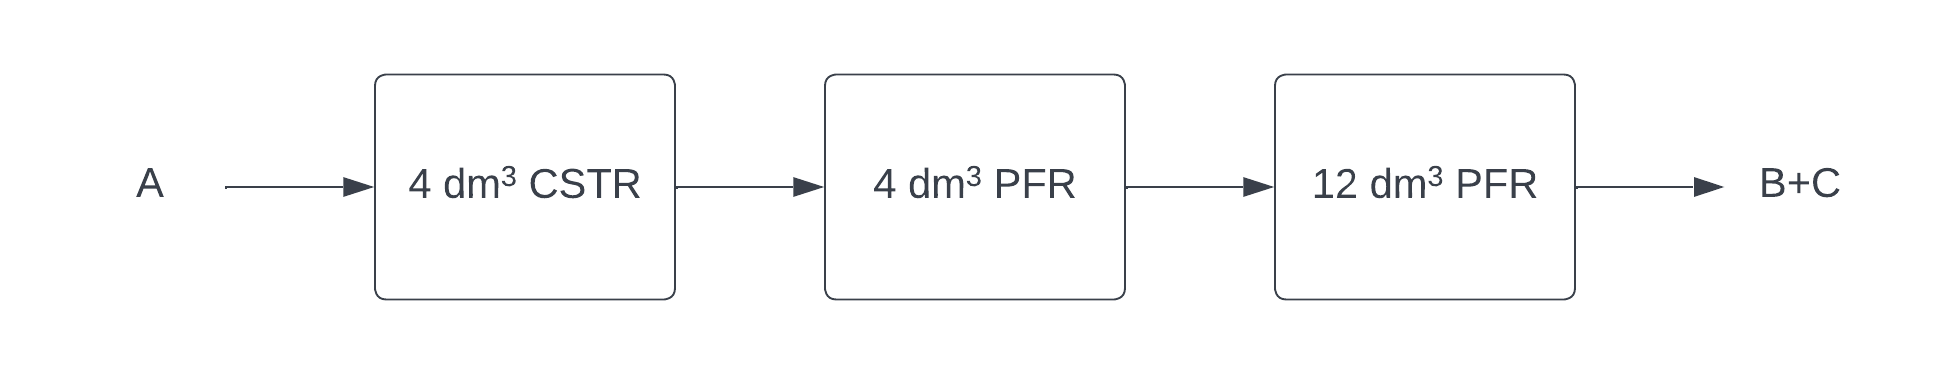
\includegraphics[scale=1]{CHEN364 P3.png}

% Problem 4
\newpage
    \item Problem 4
    \begin{align*}
        \frac{\partial x}{\partial t} &= k_1 x - k_2 x y \\
        \frac{\partial y}{\partial t} &= k_3 x y - k_4 x \\
        k_1 &= 0.02 \\
        k_2 &= 0.00004 \\
        k_3 &= 0.00004 \\
        k_4 &= 0.04
    \end{align*}
    Time range is 0 to 800 days. The initial values are $x=500$ and $y=200$.These equations are a set of coupled ODEs. The system is solved with the following code. 

    Code:
\begin{minted}[
framesep=2mm,
baselinestretch=1.2,
bgcolor=LightGray,
fontsize=\footnotesize,
breaklines,
]{python}
import numpy as np
import matplotlib.pyplot as plt
from scipy.integrate import solve_ivp, trapezoid
from matplotlib.colorbar import constrained_layout
# ODE function for Problem 4
def P_4_ODE(t, w):
    # init ode array
    f = np.zeros(len(w))
    # define x & y from input array
    x = w[0]
    y = w[1]
    # define constants
    k_1 = 0.02
    k_2 = 0.00004
    k_3 = 0.00004
    k_4 = 0.04
    # define ode system
    f[0] = k_1 * x - k_2 * x * y
    f[1] = k_3 * x * y - k_4 * y
    # return system as an array
    return f

# set initial condition
xy_initial = (500, 200)
# final time
t_final_days = 800
# solve ODE system
P_4_solution = solve_ivp(P_4_ODE, [0, t_final_days], xy_initial, method="Radau", rtol = 1e-6, atol = 1e-6)
# plotting
fig, ax = plt.subplots(2, dpi=100, constrained_layout=True, figsize=(6.4,9.6))
# solution arrays
ax[0].plot(P_4_solution.t, P_4_solution.y[0])
ax[0].plot(P_4_solution.t, P_4_solution.y[1])
# labels
ax[0].set_xlabel("Time (days)")
ax[0].set_ylabel("Number of animals")
ax[0].set_title("Problem 4 Solution")
ax[0].legend(["rabbits", "foxes"], loc="upper right")
# second plot
ax[1].plot(P_4_solution.y[0], P_4_solution.y[1])
ax[1].set_xlabel("Rabbits")
ax[1].set_ylabel("Foxes")
ax[1].set_title("Rabbits v Foxes Plot")
# save figure to image
plt.savefig(fname="P_4_figure1.png", dpi=150)
# Aggie Honor Code: An Aggie does not lie, cheat, or steal or tolerate
# those who do.
# I certify that this work is my own and not the work of another.
#
# Name: Mark Levchenko
# Assignment #: HW 1
# Question #: 4
\end{minted}
    As the rabbit population increases, the fox population increases because they have an increased food supply. However, the fox population outpaces the rabbit population, and the rabbit population declines as they become over hunted. As the rabbit population decreases, the fox population decreases as their food supply dries up. Eventually, the rabbit population declines slower than the fox population, and the rabbit population recovers. This increase followed by decline is a cycle. This cycle can be seen in the plot of the populations over time. The second plot is circular because there are two fox populations for each rabbit population, depending if the fox population is in decline or not.

    Output plots:
    
    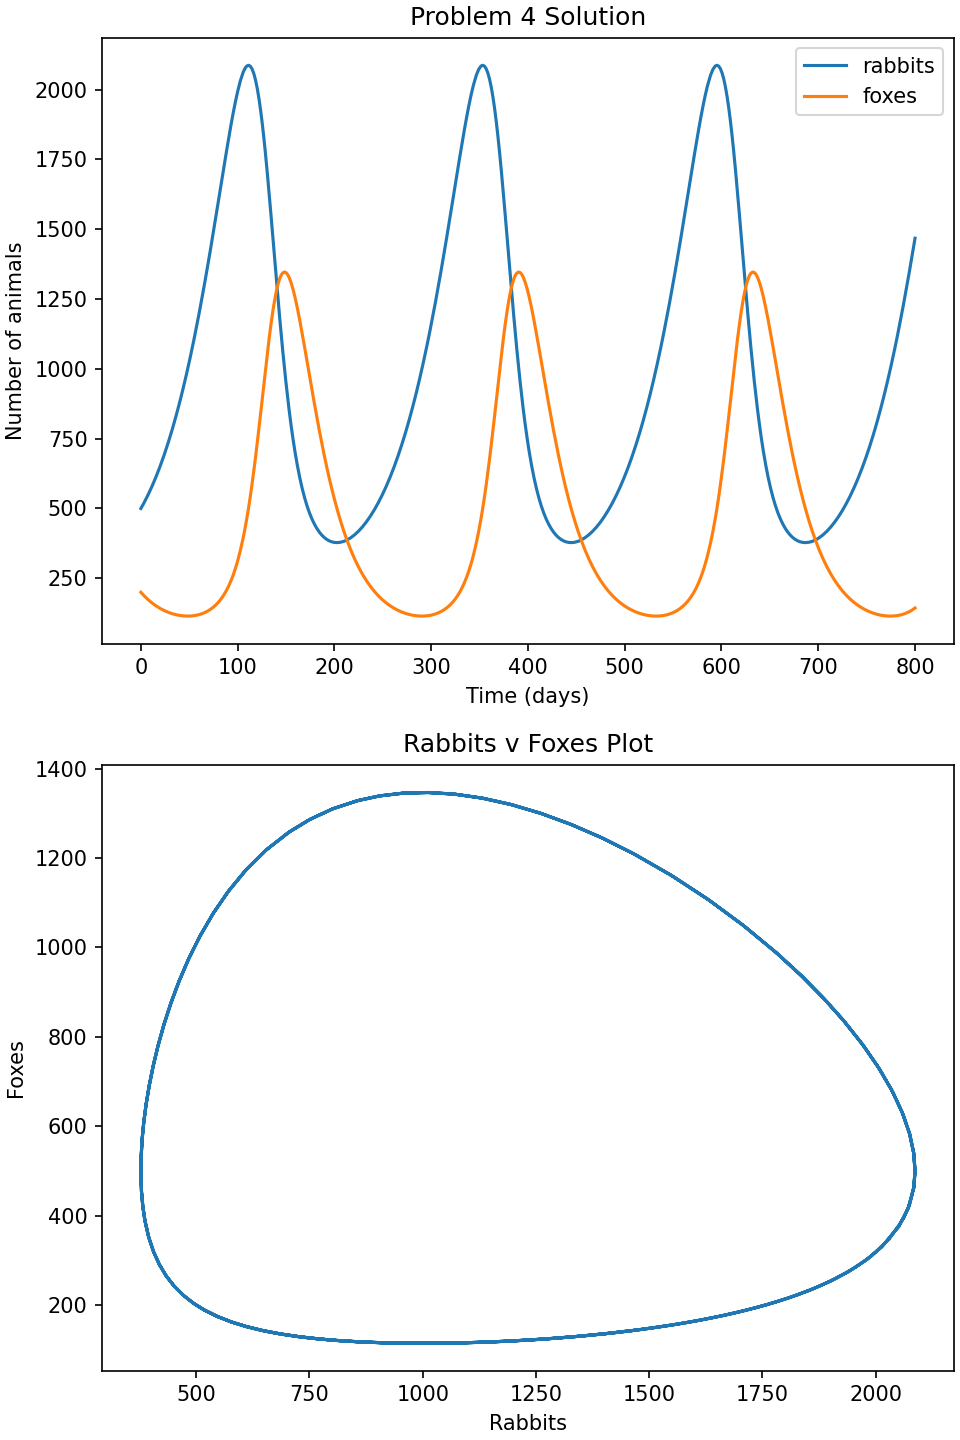
\includegraphics[scale=1]{P_4_figure1.png}

\end{enumerate}
\end{document}
